\begin{floatingfigure}[rb]{2.8in}
\vspace{-0.1in}
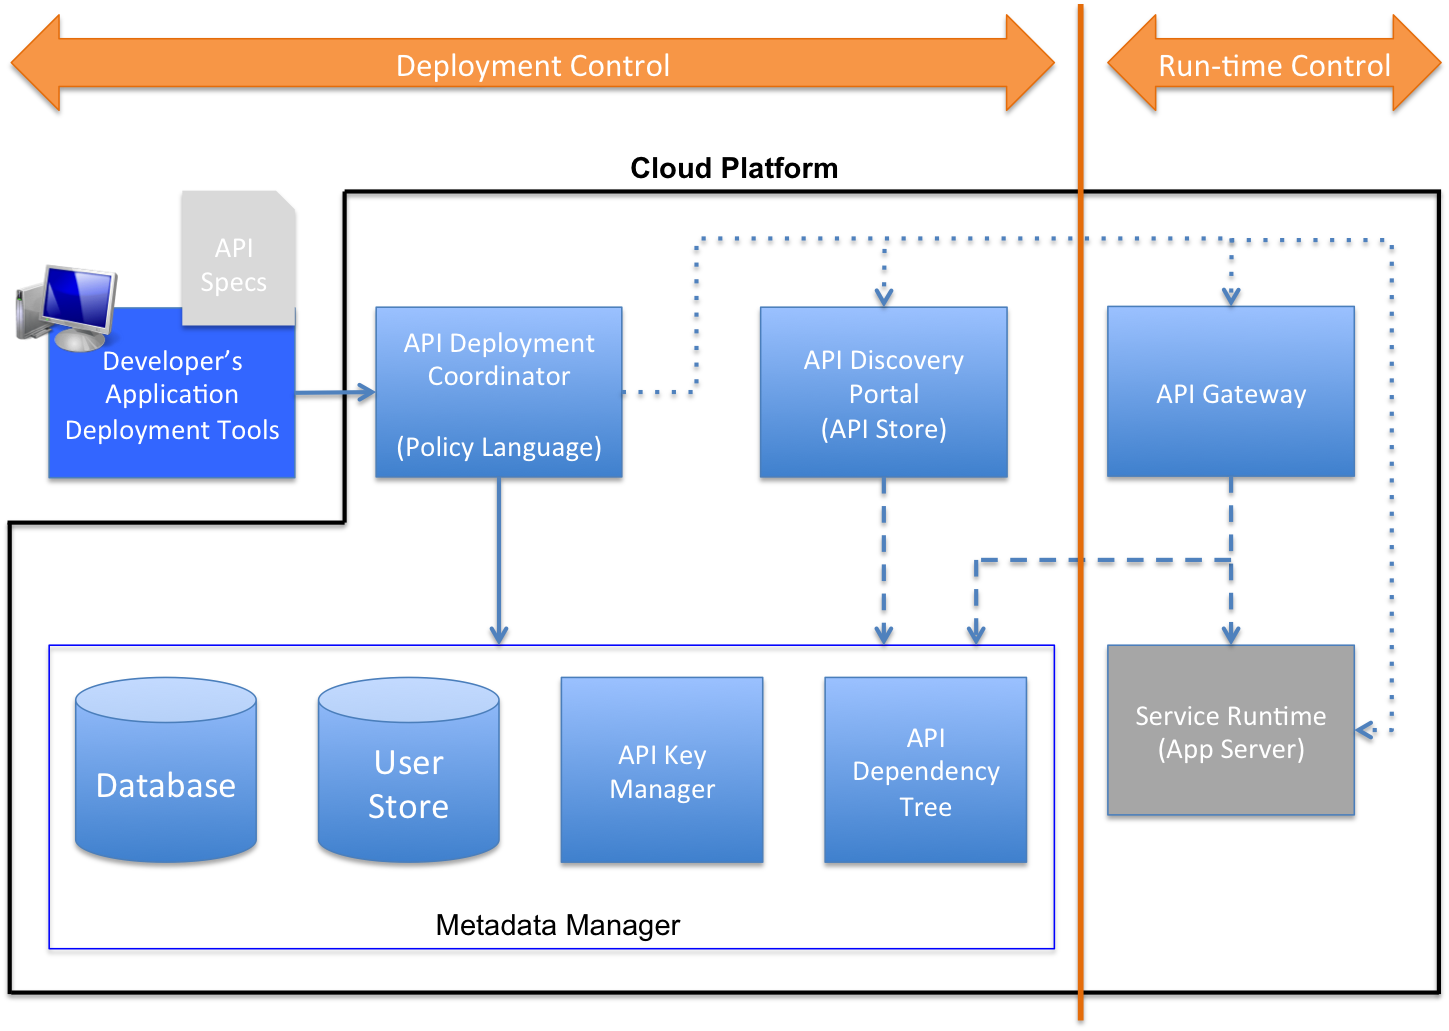
\includegraphics[scale=.27]{eager_design_2}
\vspace{-0.08in}
\caption{EAGER architecture\label{fig:eager}}
\end{floatingfigure}

I started this research with a comprehensive study on machine-readable 
API description languages. This initial survey lead me to develop a formal 
mechanism for automatically estimating the application porting effort between 
different APIs and API versions~\cite{6930607}. My algorithm takes two API descriptions 
(source API and target API) as the input, which contain axiomatic semantics~\cite{Hoare:1969:ABC:363235.363259} of 
API operations expressed in a Python-based syntax, and calculates a numeric 
value that is indicative of the effort that would be required to port an application 
from the source API to the target API. This formal approach is based on Dice 
coefficient~\cite{dice1945,738528} 
and Hoare's consequence rules~\cite{Hoare:1969:ABC:363235.363259}. The overall method has been 
validated against both randomly generated and real world API descriptions. 
I also combined my approach with $k$-means clustering in order to classify API pairs into 
multiple categories (typically 2 -- easy and hard) based on the relative difficulty in 
porting applications between them. %Initial developer studies have shown that my 
%automated mechanism closely resembles the relative difficulty 
%that human programmers associate with porting applications across web APIs.

Recently, I have further extended my automated porting effort calculation 
mechanism to also take the syntactic features of web APIs into consideration. This 
results in a two-phase API comparison algorithm where the first phase performs a 
syntactic comparison between APIs (i.e operations, input/output types), and the 
second phase performs the semantic analysis described earlier. The syntactic 
comparison is based on well-established programming languages research and 
static type checking methods.

\begin{figure}
\centering
\begin{subfigure}{.5\textwidth}
  \centering
  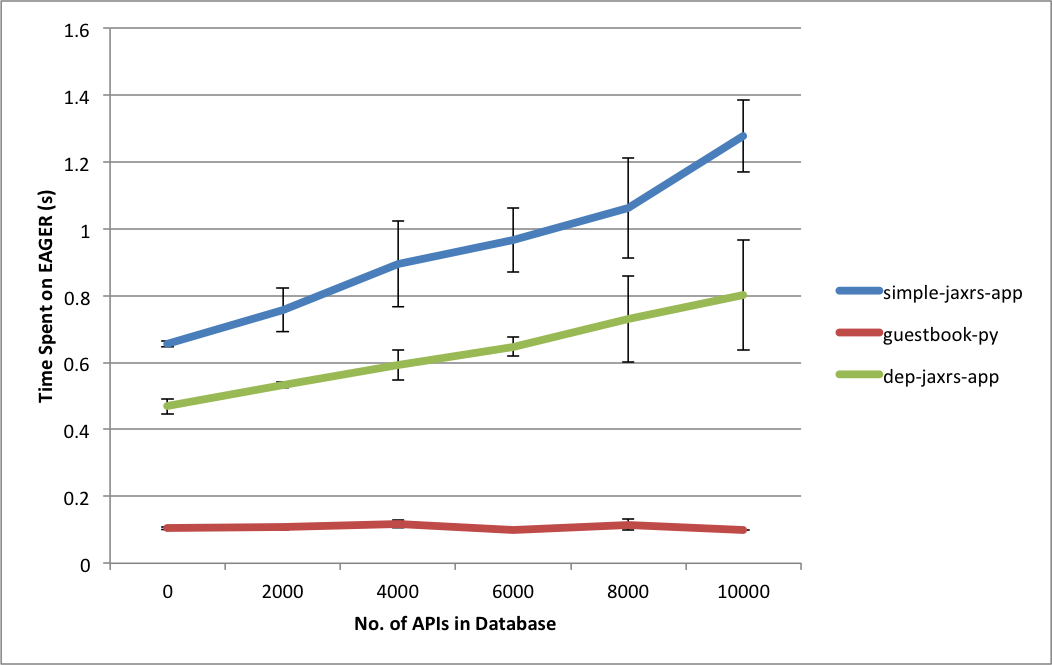
\includegraphics[width=.75\linewidth]{scalability}
  \caption{Overhead vs. number of APIs}
  \label{fig:sub1}
\end{subfigure}%
\begin{subfigure}{.5\textwidth}
  \centering
  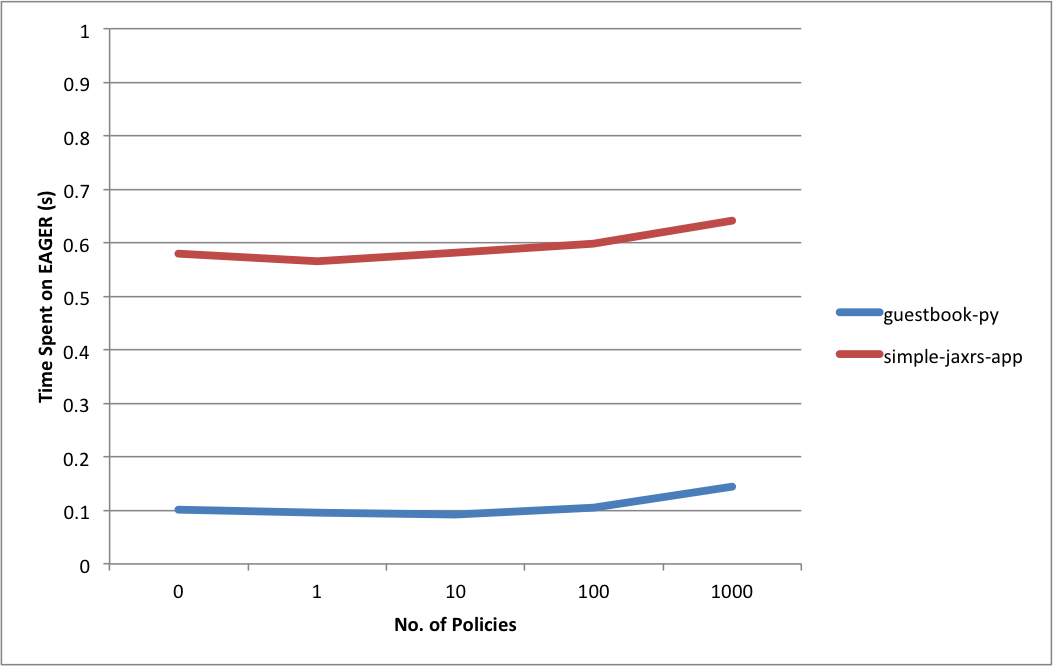
\includegraphics[width=.75\linewidth]{overhead_by_policies}
  \caption{Overhead vs. number of policies}
  \label{fig:sub2}
\end{subfigure}
\caption{EAGER performance overhead and scaling patterns}
\label{fig:eager_perf}
\end{figure}

In an effort to support design-time and run-time API governance as cloud-native features, 
I designed EAGER (Enforced API Governance Engine for REST), a 
system that augments PaaS clouds~\cite{6903538}. 
Figure~\ref{fig:eager}  shows EAGER's main components and their interactions.
The Application Deployment Coordinator intercepts all application and API 
deployment requests issued by developers, and validates them against a set of 
admin-specified policies. Applications and APIs are further subjected to a wide 
range of built-in sanity checks, which include an API backwards-compatibility test based 
on the syntactic comparison method described earlier. Applications and APIs are only 
hosted in the cloud service runtime, if all the policy and sanity checks return successfully.
Application metadata and historic information required to perform these validations are 
loaded from the Metadata Manager, which gets updated upon each successful deployment
of an application. 
We used a 
restricted subset of Python as the policy specification language, which allows programmers 
to write powerful governance policies in a very simple and intuitive way. EAGER's policy engine 
prevents all I/O operations, most third party library calls, and also global in-memory state, in 
order to perform policy validations in a stateless and side-effect free manner. EAGER also 
supports dependency management and OAuth based authorization for all deployed APIs. 
At run-time EAGER API gateway
intercepts all API calls (requests), and performs authorization and run-time policy validation.
I implemented an initial EAGER 
prototype using the AppScale~\cite{krintzappscale13} open source PaaS (open source Google App Engine clone), 
and demonstrated that EAGER adds negligible overhead to the typical application deployment 
process in the cloud, and it scales to handle thousands of APIs and policies. Figure~\ref{fig:eager_perf}
shows how the EAGER deployment overhead varies for several example web applications, under different
conditions. The run-time governance features of EAGER will be further developed and studied in
my future work.

Currently I'm conducting research in the area of automated performance analysis of web
services at development time (i.e. before services are deployed into the cloud). This was
partly inspired by EAGER, which showed that design-time governance
is not only feasible in clouds, but also desirable to run-time governance due to two reasons:

\begin{itemize}
\item APIs are designed and (re)deployed only a few times in their life cycle, whereas they might
get invoked billions of times once they are in production. Therefore, performing most governance
checks at design-time of the API avoids repeated work, and scales better in cloud environments.
\item Enforcing most governance policies and sanity checks before the APIs are in production,
prevents the overall cloud system from entering a policy non-compliant state and helps reduce
remediation costs.
\end{itemize}

\begin{floatingfigure}[rb]{2.8in}
\vspace{-0.1in}
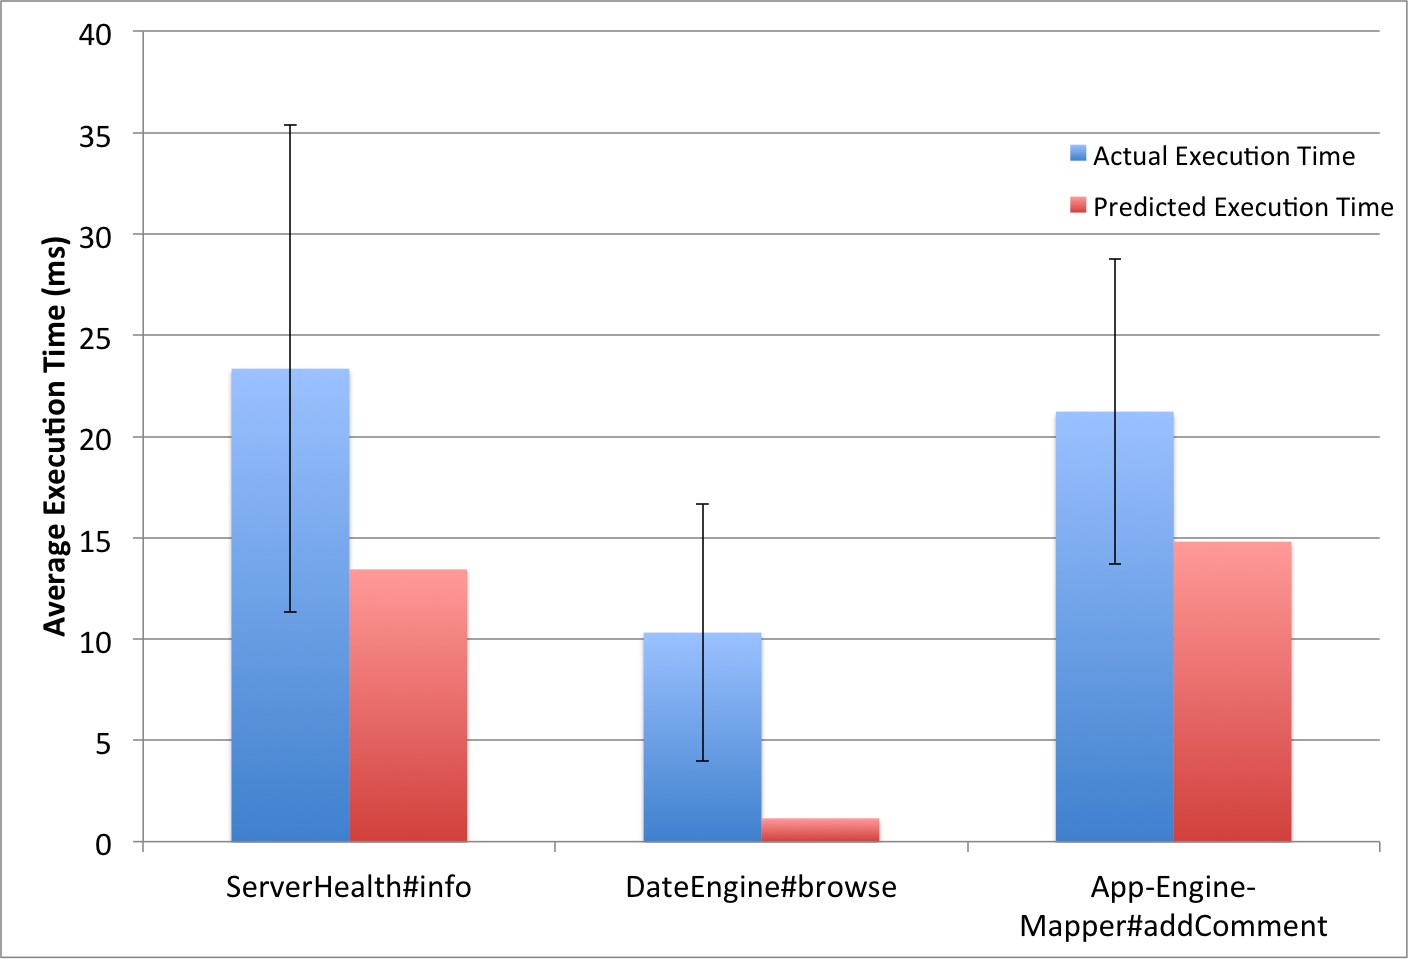
\includegraphics[scale=.27]{static_analysis}
\vspace{-0.08in}
\caption{API performance prediction results\label{fig:static_analysis}}
\end{floatingfigure}

These factors compelled me to research what other type of validations can be performed
on web services and APIs, before they are deployed in a cloud environment.
More specifically, I'm attempting to develop methods for analyzing the performance and
QoS traits of APIs at development time, in order to predict their expected performance 
levels early. This is a fairly complex research problem due to the undecidability
inherent in most program analysis tasks. However, cloud environments and SDKs
typically restrict the developers from coding arbitrary services (due to scalability reasons), 
which helps simplify the problem to some extent. Also my early survey results (conducted using
over 100 real world applications developed for PaaS clouds) show that most services developed for
clouds have very few loops and branches, making them highly amenable to static analysis and
verification.

Motivated by these early results, I'm currently using
prominent static analysis methods (abstract interpretation based loop bound analysis,
branch prediction, WCET analysis etc.~\cite{ermedahl_et_al:OASIcs:2007:1194,Yeh:1991:TAT:123465.123475,bygde2010static}) 
to compute paths of execution through service 
implementations. I use this information to build profiles of services which
specify what core cloud services and APIs are being used in a service implementation,
and in which order and frequency. My goal is to combine this information with historical
performance data of the APIs, using simulation methods or other non-parametric statistical
methods~\cite{Nurmi:2007:QQB:1791551.1791556} and derive bounds on the performance expected from the services with high
certainty. 
Such information can be used to formulate SLAs for the services or tune
the service implementations for better performance. 
I have already conducted some preliminary tests in this area using real world
Java web applications developed for the Google App Engine (and AppScale) environment,
and the initial results are quite encouraging. Figure~\ref{fig:static_analysis} shows the actual
execution time of three services and the predicted executions times of the same obtained using
a bare bones implementation of my static analysis-based approach (which is still in its infancy). 
It is interesting
to see that even without any optimizations, the predictions generated by my approach are 
within the acceptable deviation range of the actual values in two out of the three services considered.
Predictions made on the DateEngine application are somewhat off from the acceptable range, due
to its excessive use of JSP and other user interface code, which are currently not analyzed by
my static analyzer.
In the future I intend to further extend 
these methods to perform SLA management and enforcement both at design-time and run-time.